%%%%%%%%%%%%%%%%%%%%%%%%%%%%%%%%%%%%%%%%%
% Beamer Presentation

\documentclass{beamer}
\mode<presentation> {
% Theme
\usetheme{metropolis}
%\setbeamertemplate{footline} % To remove the footer line in all slides uncomment this line
%\setbeamertemplate{footline}[page number] % To replace the footer line in all slides with a simple slide count uncomment this line
%\setbeamertemplate{navigation symbols}{} % To remove the navigation symbols from the bottom of all slides uncomment this line
}

%Packages
\usepackage{graphicx} % Allows including images
\usepackage{booktabs} % Allows the use of \toprule, \midrule and \bottomrule in tables
%\usepackage{cite}
\usepackage[numbers]{natbib} % For bibliography
\usepackage{multirow}
\usepackage{hyperref}
%\usetheme{Warsaw}
\usepackage[absolute,overlay]{textpos}

% Colors
%\definecolor{Red}{rgb}{0.7,0,0}
%\definecolor{Blue}{rgb}{0,0,0.8}

% Prepare title and TOC
\title[Short title]{Introduction to R} 
\author{Marco Chiapello} 
\institute[Center for Proteomics] 
{
Center for Proteomics\\
University of Cambridge \\ 
\medskip
\textit{mc983@cam.ac.uk} 
}
\date{\today} 

%\AtBeginSection[]
%{
%\begin{frame}<beamer>
%\frametitle{Overview}
%\tableofcontents[currentsection]
%\end{frame}
%}


%-------------------------------------------
% MAIN DOCUMENT
%-------------------------------------------
\usepackage{Sweave}
\begin{document}
\Sconcordance{concordance:Rbasic_theory.tex:Rbasic_theory.Rnw:%
1 50 1 1 0 16 1 1 5 65 1}

%-------------------------------------------
% TITLE PAGE
%-------------------------------------------
\begin{frame}
	\titlepage 
\end{frame}

%-------------------------------------------
% TABLE OF CONTENTS
%-------------------------------------------
\begin{frame}{Overview}
	\small
	\tableofcontents
\end{frame}



%----------------------------------------------------------------------------------------
%	PRESENTATION SLIDES
%----------------------------------------------------------------------------------------

\section{Introduction}
\begin{frame}
	\frametitle{What R is?}
	\Large The \texttt{R} Project for Statistical Computing
	\begin{itemize}
		\small
		\item \texttt{R} is a free software environment for statistical computing and graphics
		\item Open source and cross platform (UNIX platforms, Windows and MacOS)
		\item Extensive graphics capabilities
		\item Diverse range of add-on packages
		\item Active community of developers
		\item Thorough documentation
	\end{itemize}
\end{frame}

\begin{frame}
	\frametitle{What R is?}
        \Large The \texttt{R} Project for Statistical Computing\\
	\small You can find \texttt{R} here:
	\url{https://www.r-project.org}\\
	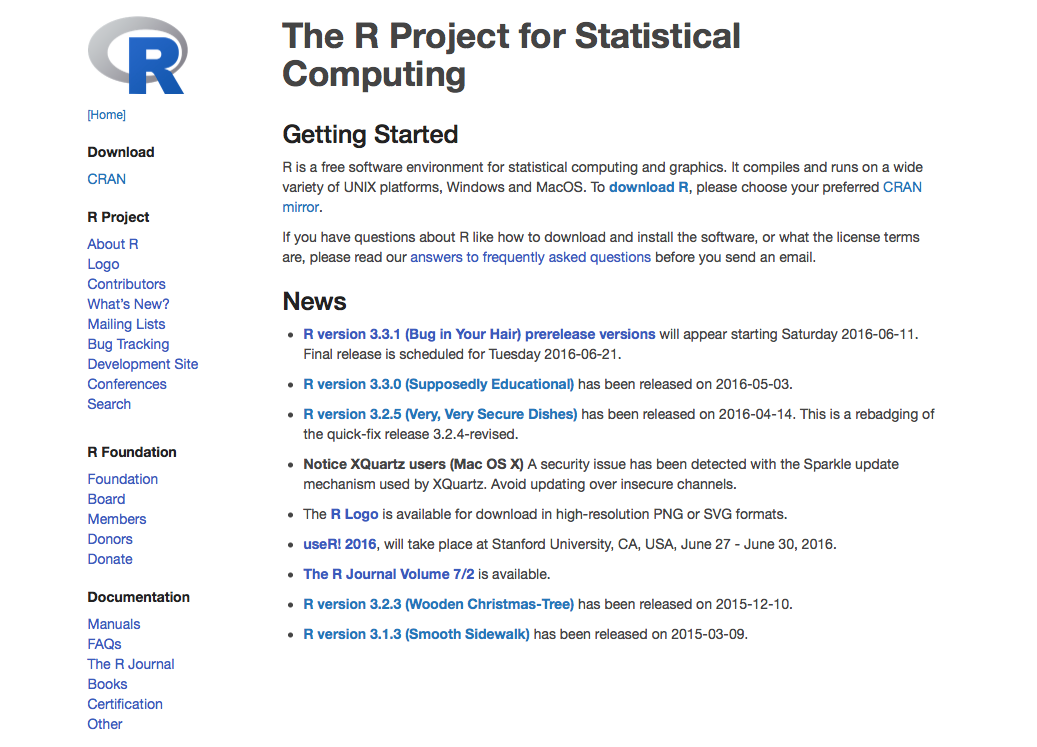
\includegraphics[scale=0.25]{figures/R-project.png}
\end{frame}

\begin{frame}
	\frametitle{What R is?}
        \Large The \texttt{R} Project for Statistical Computing\\
	\begin{itemize}
		\small
		\item R version 3.3.1 (released 2016-06-21)
		\item Currently, the CRAN {\tiny(Comprehensive R Archive Network)} package repository features 8609 available packages
			\begin{itemize}
				\item \tiny \url{https://cran.r-project.org/web/packages/available_packages_by_name.html}
			\end{itemize}
		\item Currently, the Bioconductor repository features 1211 available packages
			\begin{itemize}
				\item \tiny \url{http://www.bioconductor.org}
			\end{itemize}
		\item Executed using command line, or a graphical user interface (GUI)
		\item On this course, we use the RStudio GUI
			\begin{itemize}
				\item \tiny \url{www.rstudio.com}
			\end{itemize}
	\end{itemize}
\end{frame}

\begin{frame}
	\frametitle{Getting started}
        \Large The \texttt{R} Project for Statistical Computing\\
	\small You can find \texttt{R} here:
	\url{https://www.r-project.org}\\
	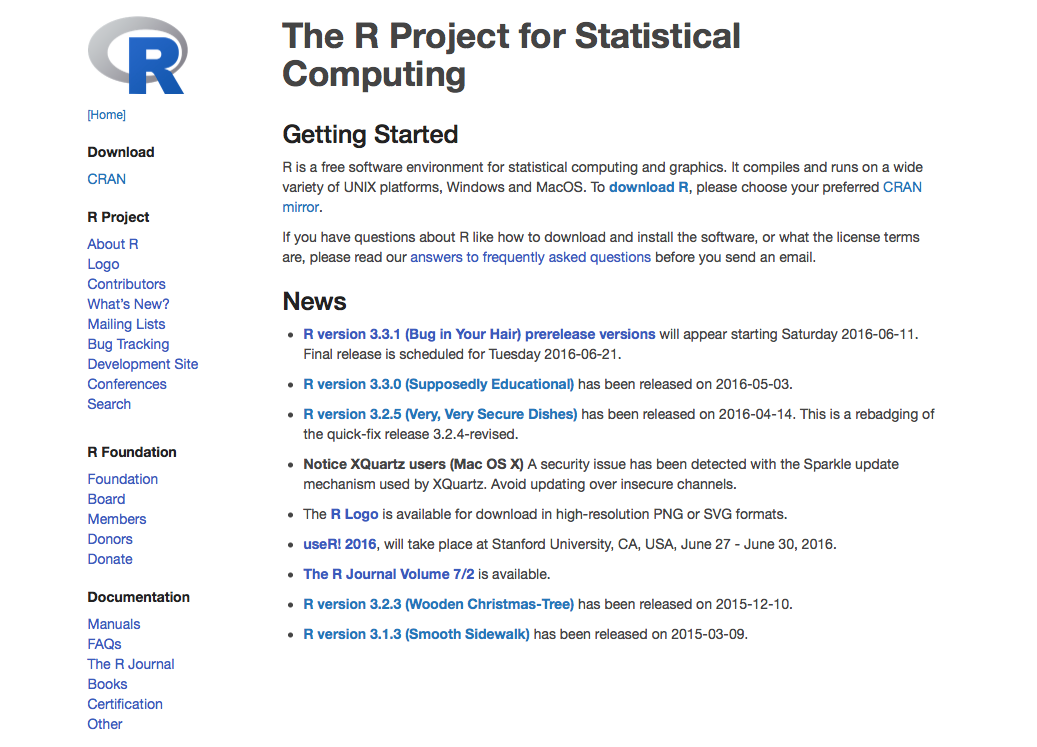
\includegraphics[scale=0.25]{figures/R-project.png}
\end{frame}







\end{document}
